\chapter{SIMULACIONES CON DISTINTOS COEFICIENTES DE DILATACIÓN ADIABÁTICA}
\label{cap:5}
Se comparan los resultados obtenidos en simulaciones del mismo problema de condición inicial pero con distinto coeficiente de dilatación adiabática $\gamma$, esto con el fin de obtener una intuición física, a través de la simulación, de cómo varía el comportamiento de un gas cuando el número de grados de libertad interno del mismo cambia.
\begin{figure}[ht]
	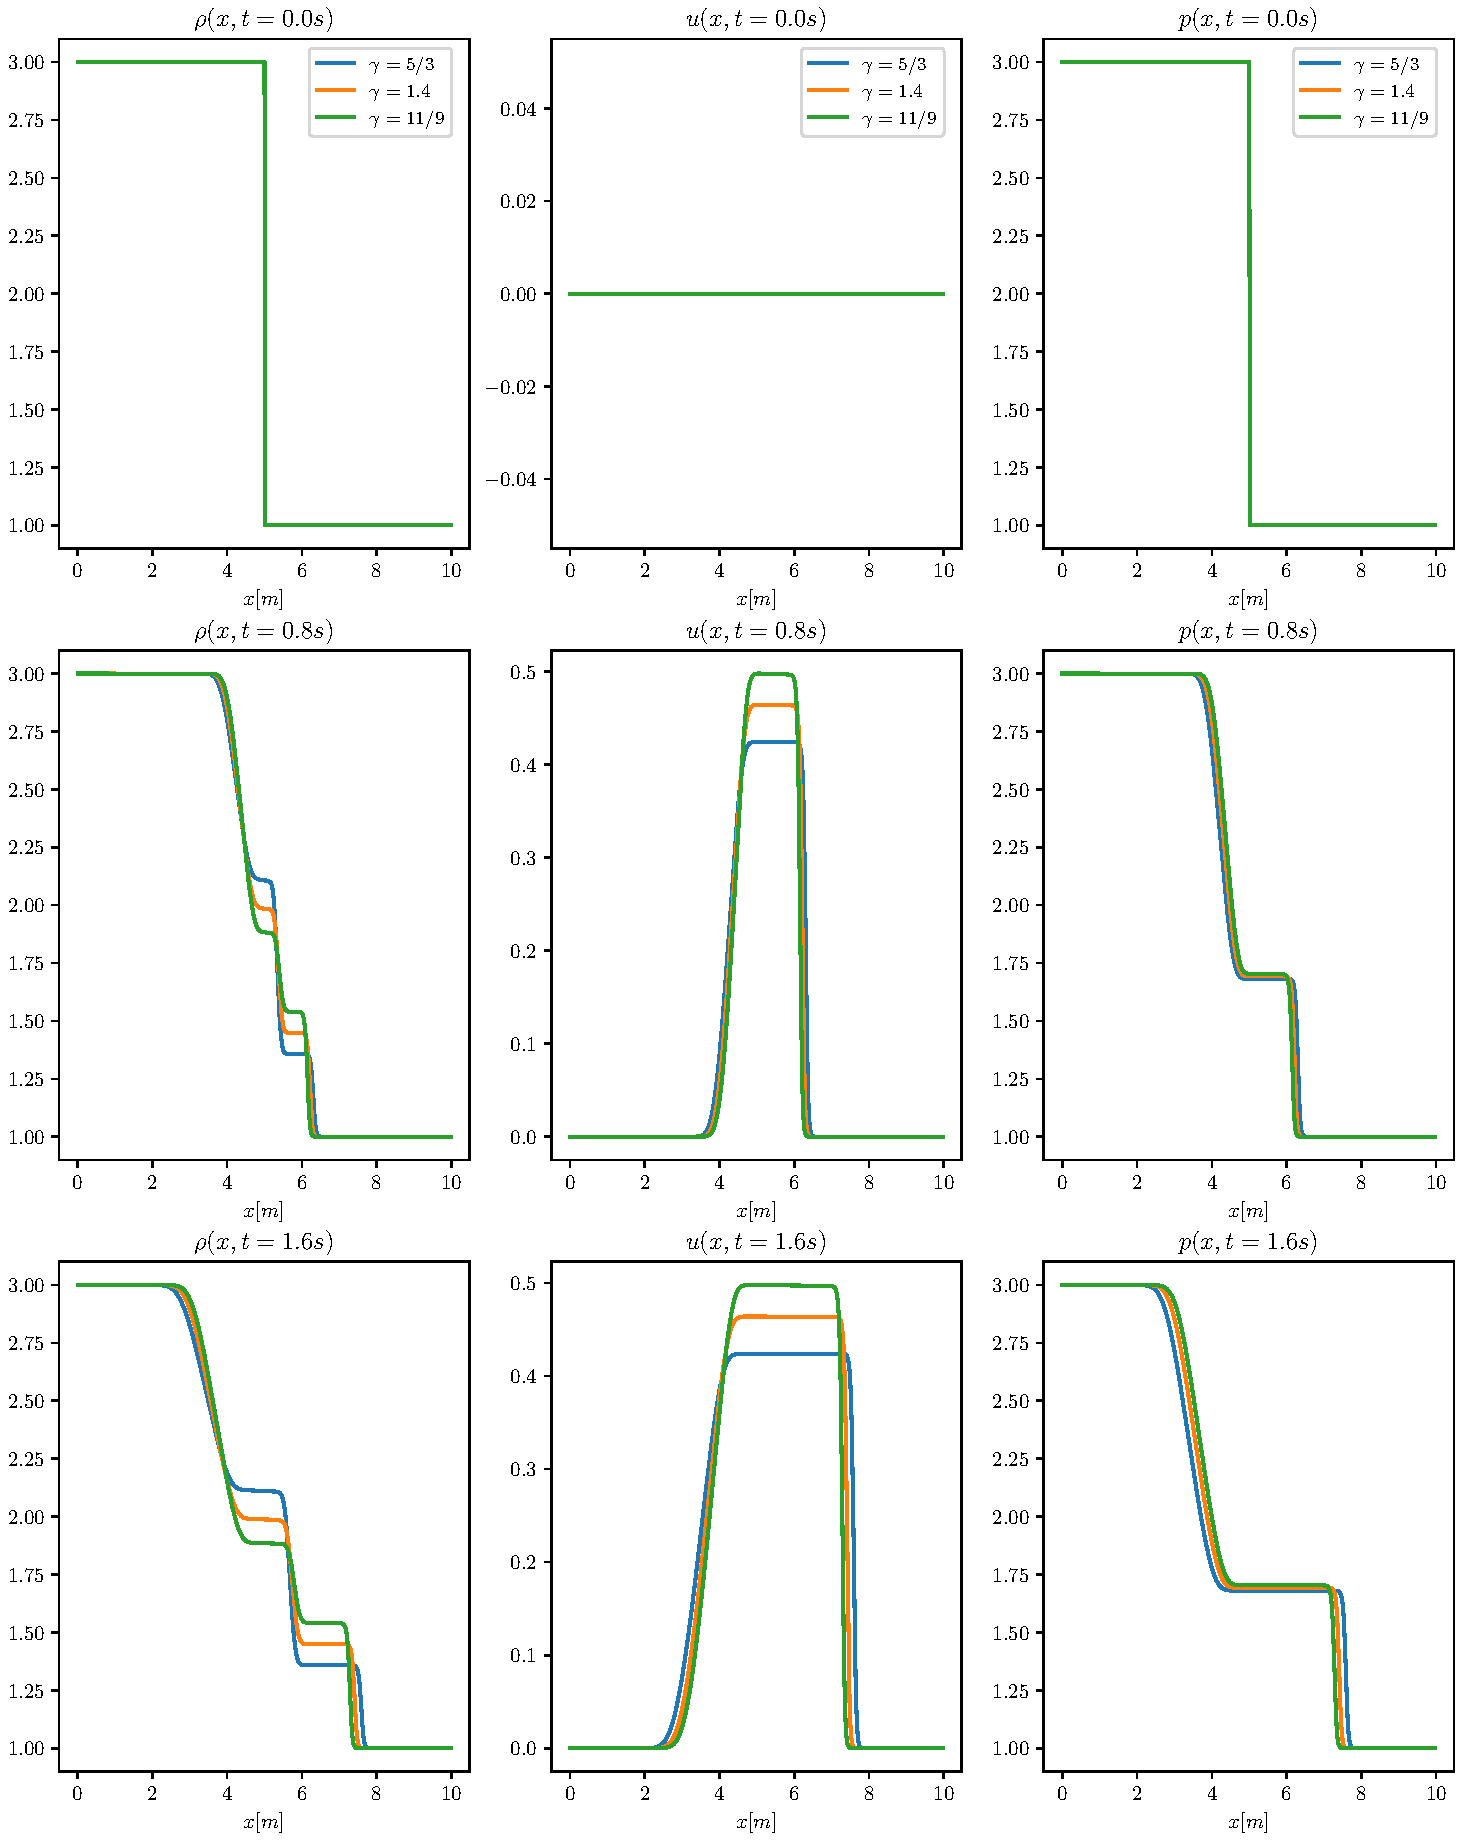
\includegraphics[width=\linewidth]{../euler1D/experimentos/graficas_sod/1.pdf}
	\caption{Primeros tres instantes de las simulaciones con distintos $\gamma$.}
\end{figure}
\begin{figure}[ht]
	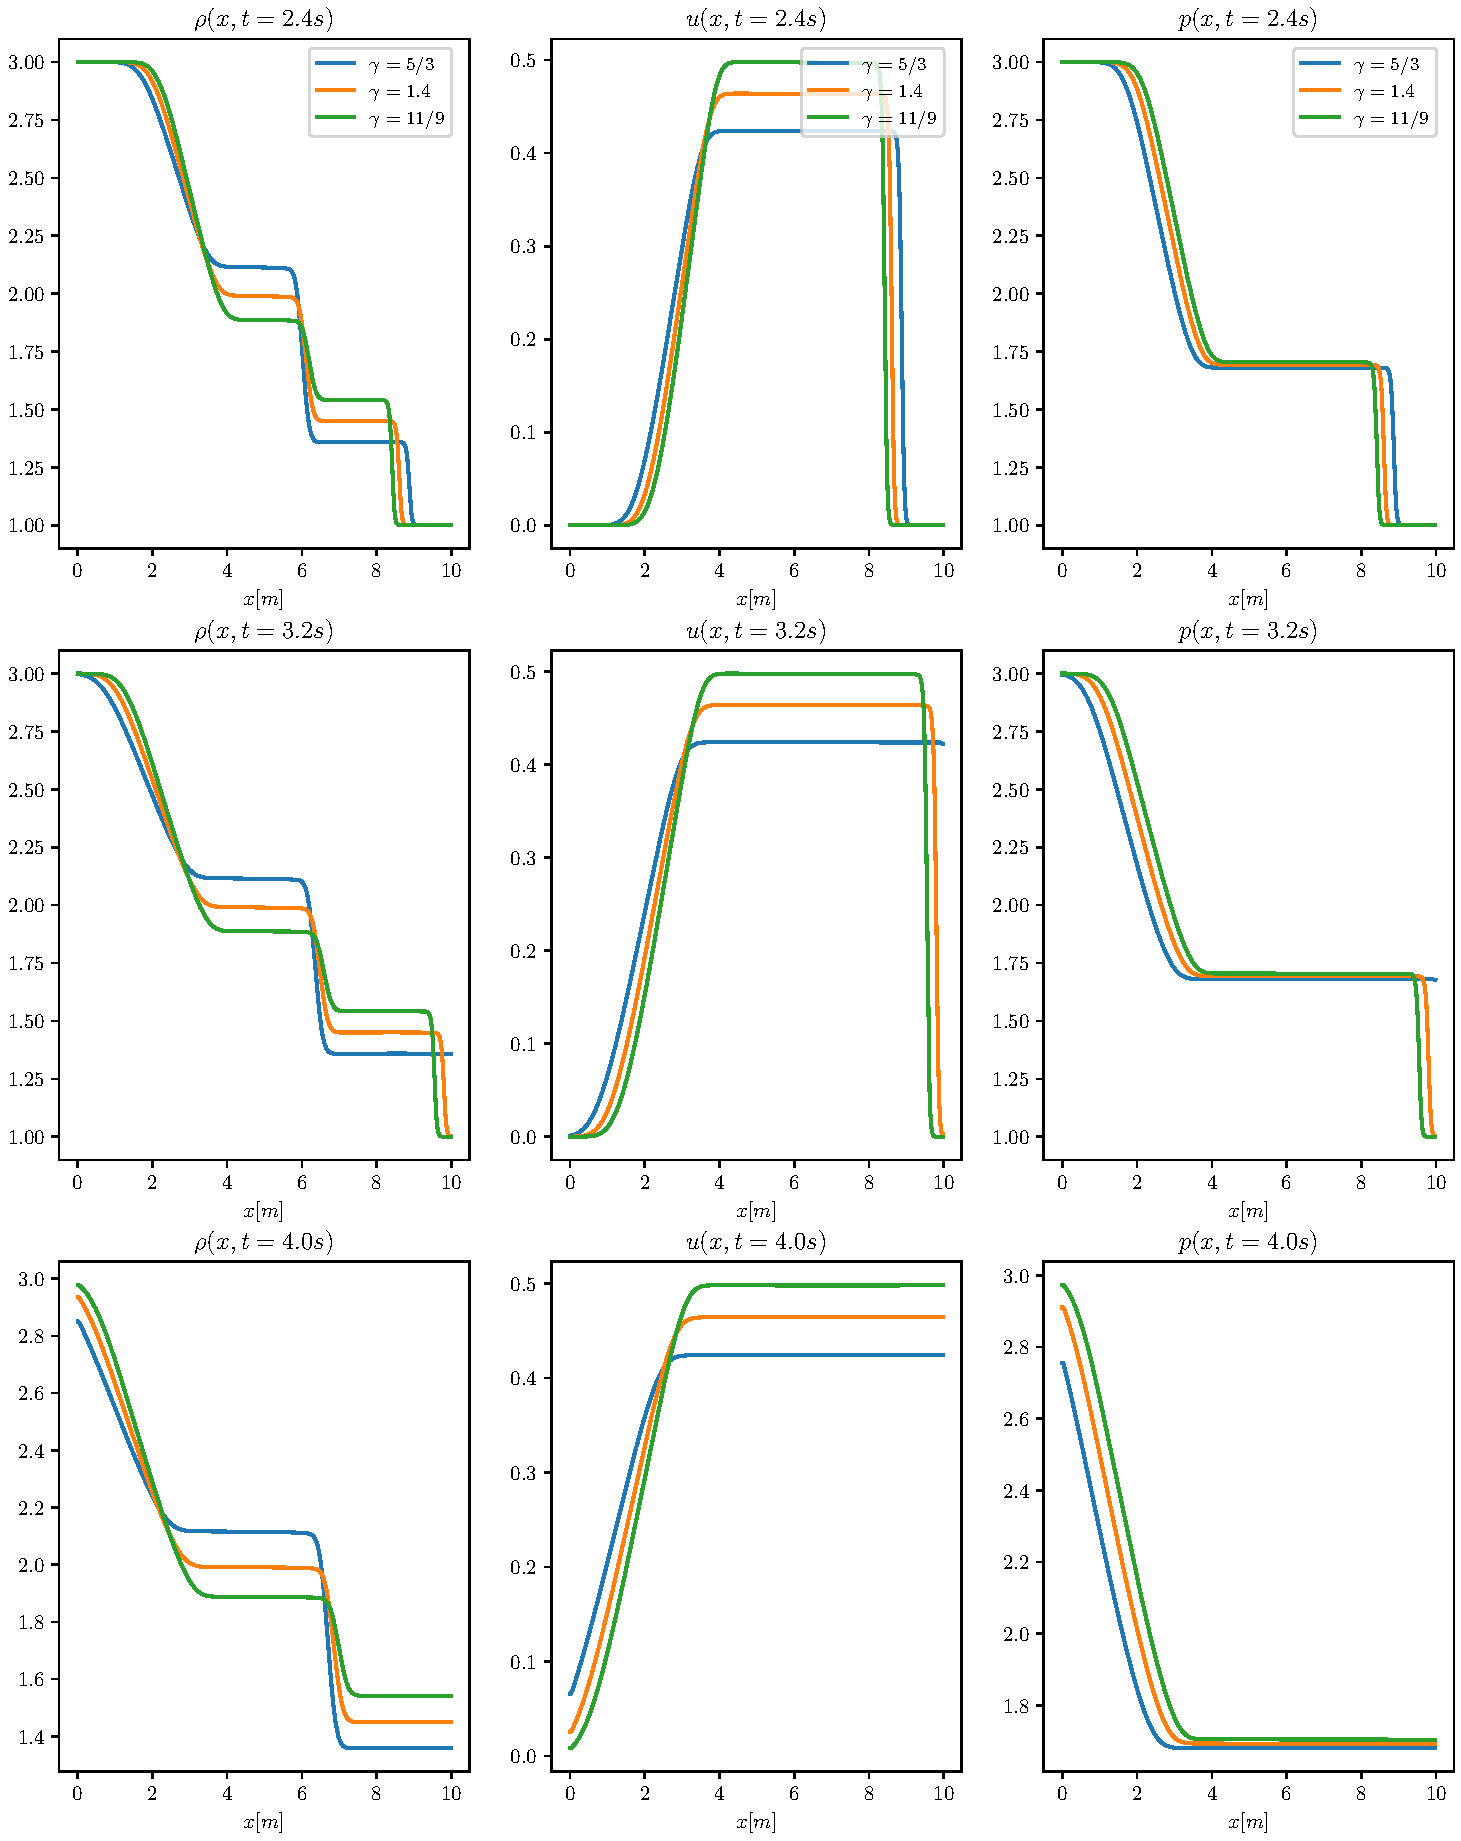
\includegraphics[width=\linewidth]{../euler1D/experimentos/graficas_sod/2.pdf}
	\caption{Últimos tres instantes de las simulaciones con distintos $\gamma$.}
\end{figure}